\documentclass[../NormeDiProgetto.tex]{subfiles}
\begin{document}
	\subsection{Sviluppo}
		\subsubsection{Scopo}
			In questa fase vengono incluse tutte le attività volte a creare il prodotto.
		\subsubsection{Aspettative}
			I risultati ottenuti in seguito ad una corretta attuazione del
			\textit{Processo di sviluppo} sono:
			\begin{itemize}
				\item Realizzare un prodotto e/o servizio che soddisfi i requisiti concordati;
				\item Realizzare un prodotto e/o servizio che soddisfi le attività di validazione
				e verifica;
				\item Determinare eventuali vincoli tecnologici e requisiti;
				\item Determinare gli obiettivi di sviluppo.
			\end{itemize}
		\subsubsection{Descrizione}
			Prendendo come riferimento lo standard [ISO/IEC 12207], si devono svolgere le seguenti
			attività:
			\begin{itemize}
				\item Analisi dei requisiti;
				\item Progettazione;
				\item Codifica.
			\end{itemize}
		\subsubsection{Analisi dei requisiti}
			\paragraph{Scopo\\}
				Determinare tutti i requisiti del progetto. Il risultato di questa attività è un
				documento in cui vengono elencati i requisiti e i relativi casi d'uso.
			\paragraph{Aspettative\\}
				Produrre il documento \analisideirequisiti\ in conformità ai requisiti richiesti
				dal Proponente.
			\paragraph{Descrizione\\}
				Vengono analizzati e tracciati tutti i requisiti attraverso l'analisi della
				specifica del capitolato e la convocazione di riunioni con il proponente
				\proponente\ volte al chiarimento di eventuali dubbi o all'approfondimento di
				requisiti già noti.
			\paragraph{Studio di Fattibilità\\}
				Alla pubblicazione dei capitolati, è compito del \responsabilediprogetto\ organizzare riunioni interne allo scopo di confrontare le opinioni dei componenti riguardo i capitolati proposti. Queste riunioni forniranno agli \analisti\ una base riguardante
				le conoscenze e preferenze di ogni membro del gruppo. È compito degli \analisti\, sulla
				base di quanto deciso, redigere uno \studiodifattibilita\ dei capitolati basandosi su:
				\begin{itemize}
					\item \textbf{Dominio tecnologico e applicativo}: conoscenza delle tecnologie richieste,
					esperienze precedenti con le problematiche poste dal capitolato, conoscenza del
					dominio applicativo;
					\item \textbf{Rapporto Costi/Benefici}: competitori e prodotti simili già presenti sul mercato
					, quantità di requisiti obbligatori, costo della realizzazione rapportato al
					risultato previsto;
					\item \textbf{Individuazione dei rischi}: Comprensione dei punti critici della realizzazione,
					individuazione di eventuali lacune tecniche o di conoscenza del dominio applicativo
					dei membri del gruppo, analisi delle difficoltà nell’individuazione dei requisiti e loro
					verificabilità.
				\end{itemize}
				Un’ultima riunione interna al gruppo \kaleidoscode\ presenterà la decisione finale sul
				capitolato scelto.
				
			\paragraph{Analisi dei requisiti\\}
				Dopo aver concluso lo studio di fattibilità, sarà compito degli \analisti redigere e/o incrementare il
				documento \analisideirequisiti.
				Lo scopo principale di questa attività è quella di produrre dei requisiti semplici e di
				facile comprensione, a partire da tutte le informazioni recuperabili.
				Per automatizzare e velocizzare il più possibile questa attività, è stato creato dal
				team il software \hyperlink{SWEgo}{SWEgo} , in cui andranno inseriti i requisiti, casi d'uso e relativo tracciamento.
				Le risorse che si possono analizzare per ottenere informazioni sui requisiti, ordinate
				per importanza in ordine decrescente, sono le seguenti:
				\begin{enumerate}
					\item Il capitolato d’appalto;
					\item Incontri con il Proponente;
					\item Incontri con il Committente.
				\end{enumerate}
			
			\paragraph{Classificazione dei requisiti\\}
				Viene stilata una lista dei requisiti individuati nel capitolato e nelle
				riunioni avvenute con il Proponente. La classificazione
				degli stessi deve avvenire secondo la seguente codifica:
				\begin{center}
					R[Importanza][Tipo][Codice]
				\end{center}
				dove:
				\begin{itemize}
					\item \textbf{Importanza} può assumere i seguenti valori:
					\begin{itemize}
						\item \textbf{0} se il requisito è obbligatorio;
						\item \textbf{1} se il requisito è desiderabile;
						\item \textbf{2} se il requisito è opzionale.
					\end{itemize}
					\item \textbf{Tipo} può assumere i seguenti valori:
					\begin{itemize}
						\item \textbf{F} se il requisito è funzionale;
						\item \textbf{Q} se il requisito è di qualità;
						\item \textbf{P} se il requisito è prestazionale;
						\item \textbf{V} se il requisito è di vincolo.
					\end{itemize}
					\item \textbf{Codice} identifica univocamente
					ciascun requisito in modo gerarchico.
				\end{itemize}
				Inoltre, per ciascun requisito deve essere indicata:
				\begin{itemize}
					\item \textbf{Fonte} dell'individuazione del requisito che può essere:
					\begin{itemize}
						\item \textbf{Capitolato};
						\item \textbf{Riunione};
						\item \textbf{Caso d'uso};
						\item \textbf{Interno} (discussioni del gruppo);
					\end{itemize}
					\item \textbf{Descrizione} breve e chiara.
				\end{itemize}
				Tutti i requisiti devono essere inseriti nell'apposito sistema di tracciamento \hyperlink{SWEgo}{SWEgo} 
				realizzato all'interno del gruppo, che provvederà alla generazione
				dei codici identificativi univoci.
				
			\paragraph{Classificazione dei casi d'uso\\}
				È richiesta agli \analisti\ l'analisi e l'identificazione dei casi d'uso, o use case (UC), procedendo dal generale al particolare,
				e il loro inserimento nel software di tracciamento \hyperlink{SWEgo}{SWEgo} .\\
				Ciascun caso d'uso sarà classificato gerarchicamente con la seguente dicitura:
				\begin{center}
					UC[Codice del padre].[Codice identificativo]
				\end{center}
				dove:
				\begin{itemize}
					\item \textbf{Codice del padre} rappresenta il codice univoco
					del relativo caso d'uso padre qualora esistesse, altrimenti è omesso;
					\item \textbf{Codice identificativo} rappresenta il codice
					univoco e progressivo del corrispondente caso d'uso. Il codice
					può includere diversi livelli di gerarchia che devono essere
					separati da un punto.
				\end{itemize}
				Inoltre, per ciascun caso d'uso deve essere indicato:
				\begin{itemize}
					\item \textbf{Nome} del caso d'uso;
					\item \textbf{Attori} coinvolti;
					\item \textbf{Descrizione} chiara e sufficientemente
					dettagliata;
					\item \textbf{Precondizione};
					\item \textbf{Scenario principale degli eventi} che descrive il principale flusso di svolgimento e l'eventuale sequenza dei casi d'uso figli;
					\item \textbf{Scenari alternativi} che descrivono la sequenza
					di eventuali casi d'uso non appartenenti allo scenario
					principale;
					\item \textbf{Requisiti} ricavati dal caso d'uso;
					\item Eventuali \textbf{Inclusioni};
					\item Eventuali \textbf{Estensioni};
					\item Eventuali \textbf{Generalizzazioni};
					\item \textbf{Postcondizione}.
				\end{itemize}
				Infine, tutti i principali casi d'uso devono essere rappresentati da un diagramma UML.\\
				Tutti i casi d'uso devono essere inseriti nell'apposito sistema di tracciamento SWEgo realizzato all'interno del gruppo, che provvederà alla generazione
				dei codici identificativi univoci.
				\paragraph{SWEgo\\}
					\hypertarget{SWEgo}
					Per effettuare il tracciamento di casi d'uso, requisiti, componenti, classi e test è stato
					scelto di realizzare un'applicazione web accessibile attraverso \gl{browser} ed ospitata
					su un server dedicato: SWEgo.
					Tale applicativo permette di aggiungere casi d'uso, attori partecipanti, requisiti, componenti,
					classi e test.
					Casi d'uso e requisiti sono automaticamente identificati attraverso i codici auto-generati
					dall'applicazione, lo stesso per componenti, classi e test;
					È inoltre possibile esportare il codice \LaTeX\ che elenca casi d'uso,
					requisiti, componenti, classi, test e le loro relazioni.
					\begin{figure} [h!]
						\centering
						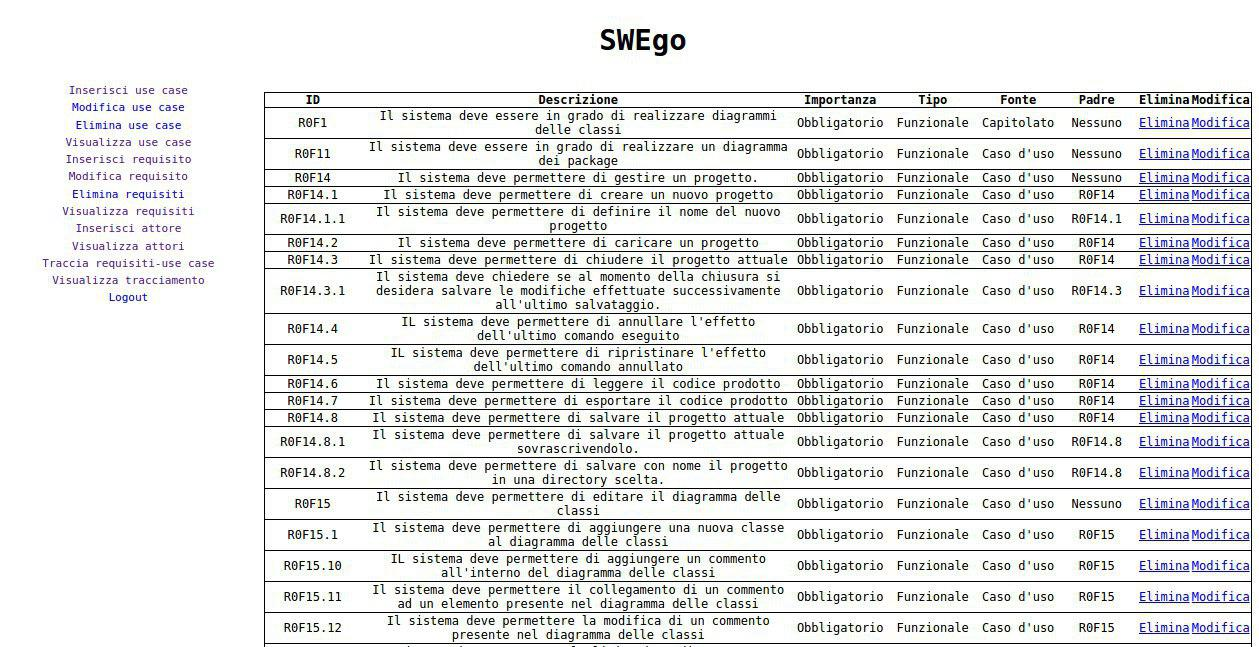
\includegraphics[scale=0.42]{./Immagini/SWEgo.jpg}
						\caption{Schermata di tracciamento requisiti in SWEgo}\label{}
					\end{figure}
		\subsubsection{Progettazione}
			\paragraph{Scopo\\}
				In questa fase viene descritta una soluzione del problema soddisfacente per tutti
				gli \gl{stakeholder}.
			\paragraph{Aspettative\\}
				I risultati ottenuti in seguito ad una corretta attuazione di tale fase sono:
				\begin{itemize}
					\item Definire l'architettura logica di sistema che identifica gli elementi
					del sistema;
					\item Definire l'architettura logica di sistema in conformità ai requisiti
					definiti;
					\item Tracciare, verificare, mantenere coerenti e sincronizzati i requisiti di sistema con
					l'architettura logica di sistema;
					\item Garantire la qualità attraverso la correttezza per costruzione.
				\end{itemize}
			\paragraph{Descrizione\\}
				Partendo dai requisiti sviluppati nella fase precedente, i \progettisti\ devono
				sviluppare l'architettura logica del sistema seguendo le sottostanti linee guida:
				\begin{itemize}
					\item Utilizzare componenti con specifiche chiare e coese;
					\item Realizzare l'architettura rispettando le risorse e i costi prefissati;
					\item Adottare strutture che si adattino al cambiamento;
					\item Utilizzare componenti riusabili;
					\item Suddividere il sistema fino a quando ogni componente ha una
					complessità trattabile;
					\item Riconoscere le componenti terminali.
				\end{itemize}
			
			\paragraph{Specifica tecnica\\}
				I \progettisti\ devono produrre la \specificatecnica, dove viene descritta la progettazione architetturale ad
				alto livello del sistema. \\ Ogni requisito deve essere tracciato
				ad un componente che lo soddisfa mediante l'apposito sistema di tracciamento \hyperlink{SWEgo}{SWEgo},
				 in modo tale da garantire
				il soddisfacimento dei requisiti.\\
				Per la progettazione ad alto livello è necessario definire i test di integrazione, sistema e
				validazione che verranno descritti nel \pianodiqualifica.
			
			\paragraph{Definizione di prodotto\\}
				I \progettisti\ devono produrre la \definizionediprodotto, dove viene descritta la progettazione di dettaglio del sistema ampliando quanto scritto nella \specificatecnica.
				Lo scopo di questo documento è quello di definire dettagliatamente ogni singola unità
				di cui è composto il sistema in modo da semplificare l’attività di codifica dei \programmatori.
				Parallelamente alla progettazione di dettaglio dei componenti software dovranno essere
				progettati i relativi test di unità che verranno descritti nel \pianodiqualifica. \\
				Ogni requisito deve essere tracciato alla/e classe/i che lo soddisfano mediante l'apposito sistema di tracciamento \hyperlink{SWEgo}{SWEgo}, in modo tale da garantire
				che ogni classe soddisfi almeno un requisito.\\
			
			\paragraph{Definizione di classe}  %%%%%%%%%%%%    TODO     %%%%%%%%%%%%%%%
				Ogni classe progettata deve essere descritta all’interno della \definizionediprodotto;
				tale descrizione deve comprendere gli attributi e i metodi con relativi parametri, una spiegazione sullo
				scopo della classe e deve specificare quale funzionalità essa modella.
				
			\paragraph{Diagrammi UML\\}
				Per definire l'architettura logica del sistema nella fase di progettazione,
				verranno utilizzati	diversi tipi di diagrammi UML 2.0:
				\begin{itemize}
					\item Diagrammi delle attività;
					\item Diagrammi delle classi;
					\item Diagrammi dei \gl{package};
					\item Diagrammi di sequenza.
				\end{itemize}
				\paragraph{Strumenti per i diagrammi UML//}	
					Per creare i diagrammi UML di package, classi, attività e sequenza relativi alla progettazione
					è stato scelto di utilizzare Astah, vista la semplice interfaccia e la presenza di una versione
					gratuitamente scaricabile.
					I diagrammi dei casi d'uso presenti nel documento \analisideirequisitiv\ sono invece generati
					automaticamente utilizzando PlantUML.
			
			\paragraph{\gl{Design pattern}\\}
				I \progettisti\ devono descrivere i design pattern utilizzati per realizzare l'architettura.
				È necessario fornire una breve descrizione ed un diagramma che ne esemplifichi il funzionamento e la struttura per ognuno di essi.
				
			\paragraph{Tracciamento}  
			\begin{itemize}
				\item Ogni requisito deve essere tracciato al componente che lo soddisfa. In questo modo sarà possibile garantire che ogni requisito venga soddisfatto e,
				al tempo stesso, misurare il progresso nell’attività di progettazione. Tale tracciamento è riportato nella \specificatecnica;
				\item Ogni test di validazione deve essere tracciato con il requisito che valida. Tale tracciamento è riportato nel \pianodiqualifica;
				\item Ogni test di sistema deve essere tracciato con il requisito che valida. Tale tracciamento è riportato nel \pianodiqualifica;
				\item Ogni test di integrazione deve essere tracciato con la componente del sistema che valida. Tale tracciamento è riportato nel \pianodiqualifica;
				\item Ogni test di unità deve essere tracciato con la classe che valida. Tale tracciamento è riportato nel \pianodiqualifica;
			\end{itemize}
		
		
		\subsubsection{Codifica}
			\paragraph{Scopo\\}
				Lo scopo della fase di codifica è quello di implementare il prodotto costruendo
				unità software eseguibili che riflettano la struttura definita in fase di
				progettazione.
			\paragraph{Aspettative\\}
				I risultati ottenuti in seguito ad una corretta attuazione di tale fase sono:
				\begin{itemize}
					\item Realizzare le unità software in conformità ai requisiti;
					\item Tracciare le unità software e le relativi componenti dell'architettura
					logica di sistema;
					\item Definire criteri di verifica delle unità software.
				\end{itemize}
			\paragraph{Descrizione\\}
				Partendo dall'architettura logica di sistema definita nella fase precedente, i
				\programmatori\ devono implementare le unità software definendone anche i criteri di
				verifica. Nello svolgimento di tali attività devono attenersi ai metodi e
				agli standard di codifica utilizzati.
			\paragraph{Standard di codifica\\}
				Ulteriori norme di codifica potrebbero essere aggiunte nelle fasi successive.
				\subparagraph{Intestazione dei file\\}
					Per i file contenenti codice si deve:
					\begin{itemize}
						\item Usare le seguente intestazione all'inizio di ogni file:\\
						\textcolor{purple}{	\\/*\\
							* File-Name: Nome del file\\
							* File-Author: Cognome Nome dell'autore\\
							* File-Date: Data di creazione\\
							* File-Summary: Breve descrizione del file\\
							* File-Description: Descrizione dettagliata del file\\
							**/}
						\item Prima di ogni classe scrivere un commento con la seguente struttura:\\
						\textcolor{purple}{	\\/*\\
							Class-Name: Nome della classe\\
							Class-Summary: Breve descrizione della classe\\
							**/}
						\item Per ogni metodo si deve scrivere un commento così strutturato:\\
						\textcolor{purple}{	\\/*\\
							Method-Name: Nome della classe\\
							Method-Summary: Breve descrizione della classe\\
							Method-Input: breve descrizione dei parametri della funzione nel caso
							ci siano\\
							Method-Output: breve descrizione dei valori di ritorno nel caso ci siano\\ 
							**/ }
					\end{itemize}
				\subparagraph{Codifica e convenzioni\\}
					Tutti i file devono seguire la convenzione UTF-8 per la codifica dei caratteri e
					LF (U+000A) per andare a capo.\\
					Per indicare il nome di variabili, classi, metodi e funzioni si deve usare la lingua
					inglese ed la notazione ``\gl{CamelCase}''. È preferibile evitare di usare nomi ambigui che
					potrebbero generare confusione.\\
					Lo stile di indentazione del codice da seguire è una variante del ``\gl{K\&R}'' dove lo stile
					di indentazione delle parentesi del corpo di una funzione è uguale a quello usato per
					i blocchi. L'indentazione deve essere effettuata utilizzando il tasto di tabulazione.\\
					È preferibile evitare lo sviluppo di metodi e funzioni ricorsive. Qualora fossero
					comunque usate si deve dimostrarne la corretta terminazione e valutarne l'impatto sulle
					performance del prodotto in termini di memoria utilizzata.\\
			\paragraph{Metriche\\}
				Nello sviluppo del codice i \programmatori\ devono tenere sotto controllo i seguenti indicatori e accertarsi che i loro valori siano conformi a quanto indicato nel \pianodiqualificav:
				\begin{itemize}
					\item \textbf{Rapporto linee di commento su linee di codice\\}
						Indica il rapporto tra linee di commento e linee di codice in un
						file (linee vuote escluse). Ritenendo importante la rapidità di
						comprensione del codice, questa metrica è utile per stimare la
						manutenibilità;
					\item \textbf{Complessità ciclomatica\\}
						Indica il numero di cammini linearmente indipendenti attraverso il
						grafo di controllo di flusso del metodo/funzione: i nodi del grafo
						corrispondono a gruppi indivisibili di istruzioni mentre gli archi
						connettono due nodi se il secondo gruppo può essere eseguito
						immediatamente dopo il primo.\\
						È possibile ridurre l'indice di complessità attraverso la
						suddivisione del metodo/funzione in più parti;
					\item \textbf{Livello di annidamento\\}
						Indica quante strutture di controllo sono inserite l'una all'interno
						dell'altra. Un alto livello di annidamento può portare ad una
						complessità maggiore del codice causando difficoltà nella verifica,
						comprensione e modifica dello stesso;
					\item \textbf{Chiamate innestate di metodi\\}
						Indica quante chiamate innestate di metodi sono inserite l'una
						all'interno dell'altra. Un alto valore può portare a una saturazione
						dello \gl{stack};
					\item \textbf{Copertura del codice\\}
						Rappresenta la percentuale di codice eseguita durante i test.
						Maggiore è questo valore, più esaurienti saranno i test e maggiori
						sono le probabilità di individuare gli eventuali errori;
					\item \textbf{Numero di linee per metodo\\}
						Indica il numero di \gl{statement} che compongono un metodo.
						Se un metodo risulta troppo lungo il suo funzionamento risulterà più
						complicato da comprendere, quindi può essere opportuno dividerlo in
						più sotto-funzioni. Un metodo troppo lungo potrebbe addirittura essere
						sintomo di cattiva progettazione della classe;
					\item \textbf{Validazione \gl{W3C}\\}
						L'applicativo web deve superare il test di validazione offerto da
						W3C con 0 errori gravi.
						Sono accettati avvisi ed inesattezze che non compromettano le
						funzionalità del sito fino a un massimo di 10 per pagina;
				\end{itemize}
\end{document}
